% !TEX TS-program = arara
% arara: xelatex: { synctex: on, options: [-halt-on-error] } 
% arara: biber
% % arara: texindy: { markup: xelatex }
% %% arara: makeglossaries
% % arara: xelatex: { synctex: on, options: [-interaction=batchmode, -halt-on-error] }
% % arara: xelatex: { synctex: on, options: [-interaction=batchmode, -halt-on-error]  }
% % arara: clean: { extensions: [ aux, log, out, run.xml, ptc, toc, mw, synctex.gz, ] }
% % arara: clean: { extensions: [ bbl, bcf, blg, ] }
% % arara: clean: { extensions: [ glg, glo, gls, ] }
% % arara: clean: { extensions: [ idx, ilg, ind, xdy, ] }
% % arara: clean: { extensions: [ plCode, plData, plMath, plExercise, plNote, plQuote, ] }
%-----------------------------------------------------------------
\documentclass[11pt]{PalisadesLakesBook}
\geomHDTV
\geomLandscape
%-----------------------------------------------------------------

%\AsanaFonts % misssing \mathhyphen; less on page than Cormorant/Garamond
%\CormorantFonts % light, missing unicode greek, needs scaling relative to monfont
\EBGaramondFonts % fewest pages
%\ErewhonFonts
%\FiraFonts % tall lines, all sans, much less per page, missing \in?
%\GFSNeohellenicFonts 
%\KpFonts
%\LatinModernFonts
%\LegibleFonts
%\LibertinusFonts
%\NewComputerModernFonts
%\STIXTwoFonts
%\BonumFonts % most pages
%\PagellaFonts

%\ScholaFonts
%\TermesFonts
%\XITSFonts

%-----------------------------------------------------------------
\togglefalse{plMath}
\togglefalse{plCode}
\togglefalse{plData}
\togglefalse{plNote}
\togglefalse{plExercise}
\togglefalse{plQuote}
\togglefalse{printglossary}
\togglefalse{printindex}
%-----------------------------------------------------------------
\title{Notes on fonts and typesetting, text and mathematics}
\author{John Alan McDonald 
(palisades dot lakes at gmail dot com)}
\date{draft of \today}
%-----------------------------------------------------------------
\begin{document}
\maketitle
\PalisadesLakesTableOfContents{7}
%-----------------------------------------------------------------
\def\sharedFolder{../../shared/}
%-----------------------------------------------------------------
\begin{plSection}{Introduction}

This is a collection of notes on font design,
typesetting (both for text and mathematics),
and possibly related layout problems. 
Partially notes on reading; 
partially my own work-in-progress analysis and implementation.
%-----------------------------------------------------------------
\begin{plSection}{Organizing thoughts}

\begin{itemize}

\item Better handwriting, rather than reproduce the best
traditional lead typesetting.

\item \emph{Question:} Compare evolution from handwriting to 
typesetting (including font development) for
math and 汉字/漢字/Hànzì/Kanji/Hanja/Chữ Nôm?\\
\citeAuthorYearTitle{MoteChu:1989:CalligraphyEABook}\\
\citeAuthorYearTitle{Kraus:1991:BrushesWithPower}
 
\item What could I (or somebody) do better
if I (they) were going to replace \TeX, \LaTeX, etc.


\end{itemize}
%-----------------------------------------------------------------
\end{plSection}%{Organizing thoughts}
%-----------------------------------------------------------------
\end{plSection}%{Introduction}
%-----------------------------------------------------------------
\begin{plSection}{Reading}
%-----------------------------------------------------------------
\begin{plSection}{Knuth}

\citeAuthorYearTitle{Knuth:1979:MathTypography}

\end{plSection}%{Knuth}
%-----------------------------------------------------------------
\begin{plSection}{Math style guides}
%-----------------------------------------------------------------
\begin{plSection}{American Mathematical Society}

\citeAuthorYearTitle{Swanson:1999:MathIntoType}

\citeAuthorYearTitle{LetourneauSharp:2017:AMSStyleGuide}

\end{plSection}%{American Mathematical Society}
%-----------------------------------------------------------------
\begin{plSection}{London Mathematical Society}

\citeAuthorYearTitle{RoddTornqkvist:2009:LMSStyleGuide}

Seems aimed at traditional kind of typesetting:
paper(?) copy marked in pencil(?)  
passed on to typesetter for formatting.

Interesting typo? on p $21$: ``$\theta$ vs $\mathscr{V}$''

Useful list of ``mathematical statement'' types.

Slanted fonts for emphasis; no italic in text;
math variables italic/roman by author's choice.

Latex commands used to communicate with typesetter.


\end{plSection}%{London mathematical Society}
%-----------------------------------------------------------------
\begin{plSection}{Oxford University Press}

\citeAuthorYearTitle{ChaundyBarrettBatey:1954:PrintingMathematics}

\end{plSection}%{Oxford University Press}
%-----------------------------------------------------------------
\end{plSection}%{Math style guides}
%-----------------------------------------------------------------
\begin{plSection}{Font design}
%-----------------------------------------------------------------
\begin{plSection}{Noordzij}

\citeAuthorTitle{Devroye:2014:Noordzij}

\citeAuthorTitle{Middendorp:2019:Noordzij}

\end{plSection}%{Noordzij}
%-----------------------------------------------------------------
\begin{plSection}{Rhatigan}
%-----------------------------------------------------------------
\begin{plSection}{The Monotype 4-line system}

\citeAuthorYearTitle{Rhatigan:2007:Monotype4Line}

\begin{plQuote}
{\citeAuthorYearTitle[p.~11]{Rhatigan:2007:Monotype4Line}}
{PostwarMonotype}
As it resumed production in the wake of the war,
Monotype found itself struggling to meet its customers'
demands for parts and equipment. 
In this climate of an uncertain return to economic stability,
it make sense that the company would choose to develop
technology such as the 4-line system that adapted to its existing
equipment and working methods, 
rather than solutions that would make unrealistic demands
on the company's ability to devise and manufacture 
new kinds of equipment altogether. 
\end{plQuote}

Seems fundamentally limited. 
No doubt a reasonable economic compromise given the technology of
the time, but not a model for high-resolution digital typesetting.
Maybe some insights for low-resolution display 
(eg two or so tens of pixels to a character box side.)
\end{plSection}%{The Monotype 4-line system}
%-----------------------------------------------------------------
\begin{plSection}{Three typefaces for mathematics}

\citeAuthorYearTitle{Rhatigan:2007:MathTypefaces}

\end{plSection}%{Three typefaces}
%-----------------------------------------------------------------
\begin{plSection}{Gina}

\citeAuthorYearTitle{Rhatigan:2007:GinaPractice}

\citeAuthorYearTitle{Rhatigan:2007:GinaSpecimen}

Tabular oldstyle figures (digits) are nice and, I think,
relatively unusual.

(\emph{Question:} any font with quasi-oldstyle digits that alternate 
ascending above x-height and dropping below baseline?
Eg, 0 rising, 1 with a descender of some kind, 2 rising, 3 with
a descender (usual for oldstyle), 4 ascending (usual is descending).
The remaining 6--9 alternate ascending/descending in most
oldstyle digit renderings.
Don't know if this would actually look good.
Might be a project for learning FontForge?)

Mathematics examples are too limited to judge, 
but operators ($\int$, $\prod$) look too small. 
(How was the math in the specimen doc typeset?)

\end{plSection}%{Gina}
%-----------------------------------------------------------------
\end{plSection}%{Rhatigan}
%-----------------------------------------------------------------
\end{plSection}%{Font design}
%-----------------------------------------------------------------
\end{plSection}%{Reading}
%-----------------------------------------------------------------

\BeginAppendices
%-----------------------------------------------------------------
\begin{plSection}{Typesetting}

This document was typeset using Mik\TeX{} $2.9$ \cite{Schenk:2017:Miktex} 
and {\TeX}works $0.6.5$ \cite{KewLoffler:2017:Texworks} 
on \textsc{Windows} $10$. 
I used \texttt{arara} \cite{CeredaEtAl:2021:Arara} 
to run \texttt{xelatex}, \texttt{biber}, \texttt{makeglossaries},  and
\texttt{texindy: { markup: xelatex }}.
I believe only Mik\TeX\  and {\TeX}works are Windows specific; 
the actual typesetting tools should be usable on Linux and MacOS as well.

See also \cite{Talbot:2012:LatexNovices,Talbot:2013:LatexPhD}.

\begin{plScreen}
{Configuring {\TeX}works for \texttt{arara}.}
{fig:arara}
\centering
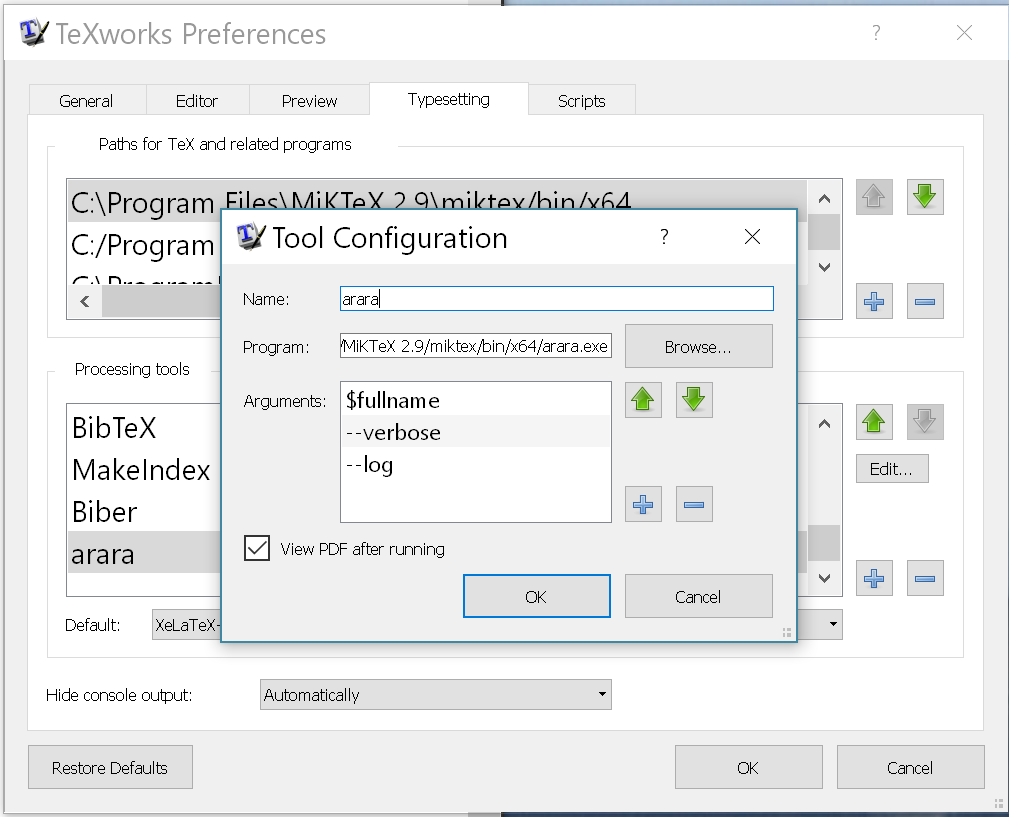
\includegraphics[scale=0.75]{../figs/arara.png}
\end{plScreen}
\vfill
\end{plSection}%{Typesetting}

%-----------------------------------------------------------------
%-----------------------------------------------------------------
\end{document}
%-----------------------------------------------------------------
